\chapter{Data Parallelism}

\begin{figure}[t]
	\centering
	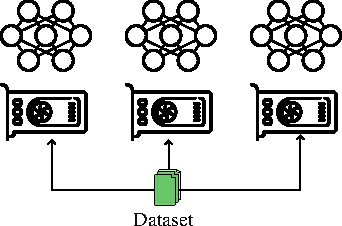
\includegraphics[scale=1.5]{./images/data_parallel.pdf}
\end{figure}

\section{Data Parallel}
\label{sec:parallelism:data_parallelism:dp}

The first step of the typical training loop for deep learning models is to split a dataset into batches so that we can feed them into the model and compute gradients corresponding to them. As the model size grows up, we couldn't fit the model into a single GPU. The \textit{data parallelism} tries to tackle the issue by clone the model across multiple GPUs so that each GPU can take a small portion of the batches for each iteration. Data Parallel (sometimes referred to as ``single-node data parallel'') is typically used when you have \textbf{multiple GPUs on a single machine}. 

Let's say the batch size is 10 and we have 5 GPUs. Then, each GPU takes 2 batches and calculate gradients by on its own. The calculated gradients are then synchronized across the GPUs pretending they are computed on a single GPU. Finally, the synchronized gradient information is going to be distributed to them. 

There are some important things to mention: 
\begin{enumerate}
	\item One process (or master thread) becomes a bottleneck for gradient aggregation and parameter updates.
	\item As you increase the number of GPUs, or try to involve multiple machines, communication overhead grows significantly and can slow down training.
	\item Each GPU holds a copy of the entire model, which can be large.
\end{enumerate}

\section{Distributed Data Parallel}
\label{sec:parallelism:data_parallelism:ddp}
To alleviate such issues, we can adopt an approach called \textit{Distributed Data Parallel} (DDP), which is designed to scale training across many GPUs, potentially across multiple machines (nodes). Modern deep learning frameworks (like PyTorch torch.nn.parallel.DistributedDataParallel) typically recommend DDP as the best practice for multi-GPU/multi-node training due to better performance and scalability. During backpropagation, gradients are shared among GPUs through efficient communication primitives, resulting in synchronized model parameters across all GPUs.

Key benefits:
\begin{itemize}
	\item Scalability: You can increase the number of GPUs (and even add more machines) to handle large datasets and bigger models.
	\item Performance: DDP typically provides better performance than older methods like \textsc{nn.DataParallel} (in PyTorch) because it uses \textit{all-reduce} and eliminates the single ``master'' bottleneck.
	\item Flexibility: You can combine DDP with other parallelization strategies (\eg model parallel, sharded data parallel, pipeline parallel) if needed.
\end{itemize}

\subsection{Concepts and Terminology}

All-Reduce is a collective communication operation commonly used in distributed computing (especially in high-performance computing and deep learning). In simple terms:
\begin{itemize}
	\item Each process (or GPU) starts with its own data (\eg local gradients).
	\item These data are combined (usually via a reduction operation like sum, mean, min, or max) across all processes.
	\item The result of that reduction (\eg the summed gradients) is then shared back so that every process receives the same reduced value.
	\item Hence the name: ``all'' (everyone gets the result) + ``reduce'' (combine data).
\end{itemize}

Basic Terms:
\begin{itemize}
	\item World Size: The total number of processes engaged in the distributed job. Often, we run one process per GPU, so world size is the number of GPUs.
	\item Rank: A unique integer ID assigned to each process. Ranks typically range from 0 to $\text{world\_size} - 1$. Rank 0 is often referred to as the ``leader'' or ``master'' process, but in DDP, every process does roughly the same work.
	\item Local Rank: When multiple GPUs reside on a single node, local rank identifies which GPU a specific process is mapped to on that local machine (\eg 0 for the first GPU, 1 for the second, etc.).
	\item Backend: The communication backend used for synchronization (\eg nccl). For GPU training, NCCL is typically recommended because it's optimized for high-performance GPU-to-GPU communication.
	\item Initialization Method: Describes how processes connect with each other (\eg a TCP store, a file-based store). This allows all processes to know who's who in the cluster.
\end{itemize}

\subsection{How DDP Works Under the Hood}
\begin{enumerate}
	\item  Process Per GPU: Each GPU runs the same script in its own process.  
	\item  Data Subset: A DistributedSampler ensures that each process sees a unique subset of data. This prevents overlap in data usage among GPUs.  
	\item  Full Model Copy: Each GPU has a full replica of the model in memory.  
		\begin{itemize}
			\item For massive models, consider \textit{Sharded DDP} (\eg PyTorch's FSDP or DeepSpeed ZeRO) to split parameters across GPUs.
		\end{itemize}
	\item  All-Reduce Gradient Sync: After backprop, gradients are summed (or averaged) across processes with an all-reduce operation. This keeps all models in sync.
\end{enumerate}




